\section{Importance Sampling}

\subsection{Implementation}

The goal of this task is to implement the Metropolis-Hastings algorithm, which generates states $\Phi_i$ form a given probability-distribution $P(\Phi_i)$ instead of weight the observable $A(\Phi_i)$ with $P(\Phi_i)$ like it is the case for the simple sampling method.
This algorithm is implemented in the file \lstinline|metropolis.py|.

\listfile{../src/metropolis.py}{src/metropolis.py}{3}{16}{Metropolis algorithm}{metro}

In order to do this the algorithm generates a new state$\Phi_{i+1}$ from the old state $\Phi_i$ via a function \lstinline@trial_move()@ in line 10.
Thereby the new state must be random in some way.
Then in the if/else-statement the new state is accepted with an probability $\Min{1,P(\Phi_{i+1})/P(\Phi_i)}$.\\

At the end the function returns a list of N+1 states and the acceptance rate $\alpha$.

\subsection{Use Metropolis for Runge Function}

Now the Metropolis algorithm should be used to generate $N=100 ,000$ samples of an scalar state $\Phi =x$ which should be distributed according to the Runge function.
Therefor the trial move should be an uniform random number in the interval $[x-\D x, x+\D x]$ with $\D x\in \lb 0.1, 1, 10, 100\rb$.\\

The trial move is implemented in \lstinline|metropolis.py|.

\listfile{../src/metropolis.py}{src/metropolis.py}{18}{23}{Trial move}{tm}

As you can see there is another function \lstinline|trial_move_set_dx| which is used to set the global variable \lstinline|tm_dx|.\\

The main loop is implemented in \lstinline@imp_samp.py@.

\listfile{../src/imp_samp.py}{src/imp\_samp.py}{12}{24}{Importance sampling}{impsamp}

In lines 7-11 the necessary variables are initialized.
You can set the initial state $x_0$ by passing \ls{--x0 <value>} when call the function. Its default value is a random number in between $-5$ and $5$.
The main for loop sets \ls{tm_dx} to $\D x$ and runs the metropolis() function for the different $\D x$.\\

As probability-distribution the function \ls{runge()} is used. 
Because of only using it in a fraction $P(\Phi_{i+1})/P(\Phi_i)$ the function must not be normalized.

\subsection{Evaluation}

\begin{figure}[ht]
	\centering
	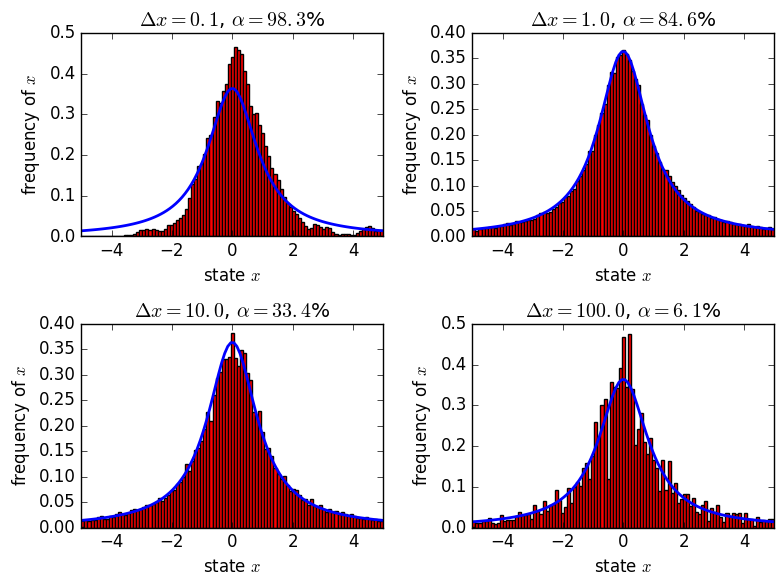
\includegraphics[width=1\textwidth]{../fig/metroplot.png}
	\caption{
		Histogram of the frequency of the states $x$ generated by the Metropolis algorithm in red.
		The blue curve is the normalized Runge function.}
	\label{metroplot}
\end{figure}

The results of the Metropolis algorithm for an initial state $x_0=0$ are shown in figure \ref{metroplot}.
This initial value is chosen because it is the most likely state.\\

As you can see steps of $\D x=0.1$ lead us to no useful distribution. 
For example values below $x=-4$ are not generated at all, what shows that the change of the state in one step is to small.
For some other tries and initial values it became even worse.
Therefore $\D x=0.1$ is to small.\\

Both $\D x=1$ and $\D x=10$ produce good distributions, but $\D x=1$ is a little better than $\D x=10$.\\

The many small peaks in the distribution for $\D x=100$ show that $\D x=100$ is to high.
The peaks come from values which did not change for a longer period because the probability to accept the new state was too low.\\

When taking a look at the acceptance rate $\alpha$ you can see that it decreases with increasing $\D x$.\\

For $\D x=0.1$ the acceptance rate is nearly $\SI{100}{\percent}$. 
This means the resulting algorithm is more or less a random walk with no respect to the given probability distribution.\\

The best result is measured for $\D x=1$ with $\alpha =\SI{84.6}{\percent}$, but also $\D x=10$ with only $\alpha =\SI{33.4}{\percent}$ produces good distributions.
Therefore it may be good to kepp the acceptance rate between $\SI{35}{\percent}$ and $\SI{85}{\percent}$.\\

$\D x=100$ produces a acceptance rate of only $\alpha =\SI{6.1}{\percent}$. 
The effects are mentioned above.

\FloatBarrier